Tabella T1 (metodo divisione):

\begin{tikzpicture}
\coordinate (0);
\foreach \t/\n[count=\i from 0,evaluate=\i as\j using int(\i+1)] in {
 K $\rightarrow$ J $\rightarrow$ I $\rightarrow$ H $\rightarrow$ G $\rightarrow$ F $\rightarrow$ E $\rightarrow$ D $\rightarrow$ C $\rightarrow$ B $\rightarrow$ A/ ,
 ,
 ,
 ,
 ,
 ,
 ,
 ,
 ,
 ,
 ,
 ,
 ,
 ,
 ,
}
\node at(\i.south)[anchor=north,draw,minimum height=1.4em,minimum width=2.5em,outer sep=0pt](\j){\n}
    node at(\j.west)[align=right,left]{\i} 
    node at(\j.east)[align=left,right,xshift=-.7em]{$\rightarrow$ \t};
\end{tikzpicture}

\vspace{20pt}
Tabella T2 (metodo moltiplicazione):

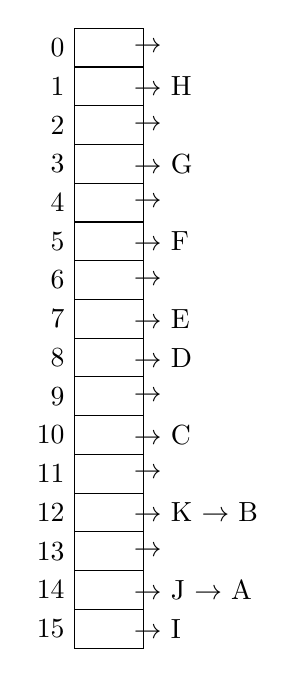
\begin{tikzpicture}
\coordinate (0);
\foreach \t/\n[count=\i from 0,evaluate=\i as\j using int(\i+1)] in {
 ,
 H/,
 ,
 G/,
 ,
 F/,
 ,
 E/,
 D/,
 ,
 C/,
 ,
 K $\rightarrow$ B/,
 ,
 J $\rightarrow$ A/,
 I/
}
\node at(\i.south)[anchor=north,draw,minimum height=1.4em,minimum width=2.5em,outer sep=0pt](\j){\n}
    node at(\j.west)[align=right,left]{\i} 
    node at(\j.east)[align=left,right,xshift=-.7em]{$\rightarrow$ \t};
\end{tikzpicture}

\newpage